\documentclass[12pt,a4paper]{article}
\usepackage[margin=2cm]{geometry}
\usepackage{xeCJK}
\usepackage{fontspec}
\setCJKmainfont{Noto Serif CJK TC}[Script=CJK]
\usepackage{amsmath,amssymb}
\usepackage{graphicx}
\usepackage{fancyhdr}
\setlength{\headheight}{14.5pt}
\addtolength{\topmargin}{-2.5pt}
\usepackage{hyperref}
\usepackage{listings}
\usepackage{enumitem}
\usepackage{titlesec}
\usepackage{caption}
\usepackage{indentfirst}
\usepackage{booktabs}
\usepackage{longtable}
\usepackage{multirow}
\usepackage{array}
\usepackage{tabularx}
\usepackage{float}
\usepackage{minted}
\setlength{\parindent}{2em}
\pagestyle{fancy}
\fancyhf{}
\cfoot{\thepage}
\linespread{1.3}
\setminted{
    linenos,                % 行號
    frame=lines,            % 上下框線
    framesep=5pt,           % 程式碼與邊框距離
    numbersep=8pt,          % 行號與程式碼距離
    fontsize=\scriptsize,   % 字體大小
    breaklines,             % 自動換行
    tabsize=4,              % tab 寬度
    rulecolor=\color{black},% 框線顏色
    xleftmargin=1.5em       % 左側縮排
}

\title{Time Frequency Analysis and Wavelet Transforms Homework 3}
\author{B12508026戴偉璿}
\date{\today}

\begin{document}

\maketitle

\lhead{TFW HW 3}
\rhead{B12508026戴偉璿}

\begin{enumerate}

%=====================================================================
\item
\begin{enumerate}[label=(\alph*)]
  \item The Fourier basis $\varphi_m(t)=e^{j2\pi f_mt}$ has only one parameter $f_m$ and is infinitely long on the $t$-axis. The 3-parameter atom
  \[
  \varphi_{t_0,f_0,\sigma}(t)=\frac{2^{1/4}}{\sigma^{1/2}}\,e^{j2\pi f_0t}\exp\!\Big(-\frac{\pi(t-t_0)^2}{\sigma^2}\Big)
  \]
  has two more parameters: $t_0$ (central time) and $\sigma$ (scaling factor). The advantages are:
  \begin{itemize}
    \item \textbf{Localized in both time and frequency.} The STFT of a Fourier basis is a horizontal line over the whole $t$-axis, while that of an atom is a small block on the time-frequency plane. Thus the coefficient $a_{t_0,f_0,\sigma}$ tells \emph{when} and \emph{which frequency} the energy appears, so it can describe signals whose frequency varies with time. The FT only tells which frequencies exist.
    \item \textbf{Adjustable scale.} $\sigma$ can match the duration of each component (small $\sigma$ for short components, large $\sigma$ for long ones), instead of a single fixed resolution.
    \item \textbf{Sparser representation.} The atoms form an over-complete, non-orthogonal basis set, and the coefficients are determined by matching pursuit. For a fixed number of terms $M$, the error $\int|x(t)-\sum_{m=1}^{M}a_m\varphi_m(t)|^2dt$ can be much smaller than that of the Fourier series. For example, a short tone burst needs only one atom but many Fourier terms.
  \end{itemize}

  \item The generalized spectrogram is
  \[
  SP_{x,w_1,w_2}(t,f)=G_{x,w_1}(t,f)\,G^*_{x,w_2}(t,f),\qquad
  G_{x,w_i}(t,f)=\int w_i(t-\tau)x(\tau)e^{-j2\pi f\tau}d\tau .
  \]
  The original spectrogram uses $w_1=w_2$, so it must trade off between the time and the frequency resolution: a wider window gives better frequency resolution but worse time resolution, and vice versa.

  In the generalized spectrogram, $w_1$ can be chosen as a \textbf{wider} window (concentrated along the $f$-axis) and $w_2$ as a \textbf{narrower} window (concentrated along the $t$-axis). The product is large only where both are large, so \textbf{both the time and the frequency resolution are improved}, i.e., higher clarity than the Gabor transform with any single $\sigma$.

  Moreover, it is the product of two linear transforms, so there are no serious cross terms as in the WDF, and the cost is only two Gabor transforms. It can be further generalized as $G^{\alpha}_{x,w_1}\overline{G^{\beta}_{x,w_2}}$ or $|G_{x,w_1}|^{\alpha}|G_{x,w_2}|^{\beta}$ to adjust the weights.
\end{enumerate}

%=====================================================================
\item \textbf{(c) $10+f^{0.6}$ is the best choice.}

The general form of the S transform is
\[
S_x(t,f)=|s(f)|\int x(\tau)\exp\!\big[-\pi(t-\tau)^2s^2(f)\big]e^{-j2\pi f\tau}d\tau .
\]
Since $\exp(-\pi t^2s^2(f))\approx0$ for $|t|>1.9/s(f)$, the window width is proportional to $1/s(f)$. $s(f)$ should \textbf{increase with $f$}, so that a wider window (better frequency resolution) is used for low frequencies and a narrower window (better time resolution) for high frequencies. Also, $s(f)$ must be positive and nonzero; otherwise the window becomes infinitely wide.
\begin{enumerate}[label=(\alph*)]
  \item $f^{1.2}$: It increases with $f$, but $s(0)=0$, so the window width $1/s(f)\to\infty$ at low frequencies, which gives very poor time resolution and cannot be implemented with a finite window. Moreover, it grows faster than $f$, so the window at high frequencies is too narrow, and the frequency resolution is even worse than the original S transform ($s(f)=|f|$).
  \item $1+\sin(f^{0.6})$: It is not monotonic. It oscillates with $f$, and $s(f)=0$ when $\sin(f^{0.6})=-1$. The resolution changes irregularly with frequency, which is meaningless.
  \item $10+f^{0.6}$: $s(f)\ge10>0$, so the window width is bounded even at low frequencies. It increases monotonically with $f$, and since $f^{0.6}$ grows slower than $f$, the frequency resolution at high frequencies is not degraded as seriously as $s(f)=f$.
\end{enumerate}
(For $f<0$, $|f|$ is used.)

%=====================================================================
\item The LCT is a twisting operation for the WDF:
\[
W_{X_{(a,b,c,d)}}(au+bv,\;cu+dv)=W_x(u,v),\qquad ad-bc=1,
\]
i.e., the point $(u,v)$ of the original WDF is moved to $\begin{bmatrix}a&b\\c&d\end{bmatrix}\begin{bmatrix}u\\v\end{bmatrix}$.

Let $(2,2)\mapsto(3,2)$ and $(2,-2)\mapsto(4,0)$:
\[
\begin{cases}2a+2b=3\\2a-2b=4\end{cases}\Rightarrow a=\tfrac74,\ b=-\tfrac14,\qquad
\begin{cases}2c+2d=2\\2c-2d=0\end{cases}\Rightarrow c=\tfrac12,\ d=\tfrac12 .
\]
Check: $ad-bc=\frac78+\frac18=1$, and $(-2,2)\mapsto(-4,0)$, $(-2,-2)\mapsto(-3,-2)$, which match the right figure. Therefore,
\[
\boxed{\{a,b,c,d\}=\Big\{\tfrac74,\;-\tfrac14,\;\tfrac12,\;\tfrac12\Big\}}
\]
Note: since the original WDF is a square centered at the origin, it is unchanged after a $90^\circ$ rotation (FT). Thus matching the corners in other orders also gives valid answers: $\{\frac14,\frac74,-\frac12,\frac12\}$, $\{-\frac74,\frac14,-\frac12,-\frac12\}$, and $\{-\frac14,-\frac74,\frac12,-\frac12\}$, all satisfying $ad-bc=1$.

%=====================================================================
\item Let $g(t)=x(dt+e)$ and $y(t)=e^{j\phi(t)}g(t)$, where $\phi(t)=at^3+bt^2+ct$.

\textbf{Step 1 (shifting and dilation):}
\[
W_g(t,f)=\frac1{|d|}W_x\Big(dt+e,\;\frac fd\Big).
\]

\textbf{Step 2 (generalized shearing):} multiplying by $e^{j\phi(t)}$ shifts the WDF along the $f$-axis by the instantaneous frequency $\phi'(t)/2\pi$:
\[
W_y(t,f)\cong W_g\Big(t,\;f-\frac{\phi'(t)}{2\pi}\Big)=\frac1{|d|}W_x\Big(dt+e,\;\frac{f-\phi'(t)/2\pi}{d}\Big).
\]
Hence the support of $W_y$ is
\[
0\le dt+e\le3,\qquad 0\le\frac{f-\phi'(t)/2\pi}{d}\le3 .
\]

\textbf{Time range:} $t\in[1,10]$ in the right figure. With $d>0$:
\[
d\cdot1+e=0,\quad d\cdot10+e=3\ \Rightarrow\ d=\tfrac13,\ e=-\tfrac13 .
\]

\textbf{Frequency range:} $0\le f-\phi'(t)/2\pi\le3d=1$, i.e., the width is $1$, which matches $(1,1)\to(1,2)$ and $(10,1)\to(10,2)$. The lower boundary $f=\phi'(t)/2\pi$ is the parabola through $(1,1)$, $(\frac{11}2,0)$, $(10,1)$ with vertex $(\frac{11}2,0)$:
\[
\frac{\phi'(t)}{2\pi}=k\Big(t-\frac{11}2\Big)^2,\qquad k\cdot\frac{81}4=1\ \Rightarrow\ k=\frac4{81}.
\]
Then
\[
\phi'(t)=3at^2+2bt+c=\frac{8\pi}{81}\Big(t^2-11t+\frac{121}4\Big)
\ \Rightarrow\ a=\frac{8\pi}{243},\ b=-\frac{44\pi}{81},\ c=\frac{242\pi}{81}.
\]
Therefore,
\[
\boxed{a=\tfrac{8\pi}{243}\approx0.1034,\quad b=-\tfrac{44\pi}{81}\approx-1.7065,\quad c=\tfrac{242\pi}{81}\approx9.3860,\quad d=\tfrac13,\quad e=-\tfrac13}
\]
Note 1: since $\phi(t)$ has a $t^3$ term, the generalized shearing of the WDF is only an approximation, so the location of the WDF is described by the instantaneous frequency $\phi'(t)/2\pi$.

Note 2: if $d<0$, then $d=-\frac13$, $e=\frac{10}3$, and $f-\phi'(t)/2\pi\in[-1,0]$. The lower boundary becomes $\phi'(t)/2\pi-1$, which gives the same $a,b$ and $c=\frac{242\pi}{81}+2\pi=\frac{404\pi}{81}$. This is also a valid answer.

%=====================================================================
\item
\begin{enumerate}[label=(\alph*)]
  \item \textbf{FRFT vs.\ FT for filter design.}
  \begin{itemize}
    \item Using the FT can only filter the noises that do not overlap with the signals \textbf{in the frequency domain (1-D)}, i.e., the cutoff lines must be horizontal. In contrast, using the FRFT can filter the noises that do not overlap with the signals \textbf{on the time-frequency plane (2-D)}.
    \item The FRFT rotates the time-frequency distribution by an angle $\phi$, so cutoff lines with \textbf{any slope} can be used (the order of the FRFT is determined by the slope). It is suitable for removing chirp noises $e^{j(n_2t^2+n_1t)}$, which overlap with the signal in the frequency domain and cannot be removed by the FT.
    \item The FRFT has a fast algorithm with complexity $O(N\log N)$, the same order as the FT.
  \end{itemize}

  \item \textbf{Generalized modulation for filter design.} Multiplying the signal by $e^{-j\phi(t)}$, where $\phi(t)=\sum_k a_kt^k$ is an arbitrary (higher-order) polynomial, shifts the time-frequency distribution along the $f$-axis by $-\phi'(t)/2\pi$ (generalized shearing). Therefore:
  \begin{itemize}
    \item A \textbf{curved} signal or noise component can be flattened to a horizontal one, and then separated by a conventional lowpass/bandpass filter. Finally, multiply back by $e^{j\phi(t)}$.
    \item The FRFT can only handle straight cutoff lines (chirps), while the generalized modulation can handle \textbf{non-linear cutoff curves}. Thus it can remove noises with higher-order phases $e^{j(n_kt^k+\cdots+n_1t)}$, e.g., denoising vocal signals whose pitch varies with time.
    \item It only needs a multiplication by a phase function plus conventional FT filtering, so the implementation is simple and the cost is low.
  \end{itemize}
\end{enumerate}

%=====================================================================
\item For white noise, $R_x(t,\tau)=E[x(t+\frac\tau2)x^*(t-\frac\tau2)]=\sigma\delta(\tau)$, which is equivalent to
\[
E[W_x(t,f)]=\sigma \quad\text{(a constant independent of $t$ and $f$)}.
\]
Thus we check whether $E[W_y(t,f)]$ is still a constant.
\begin{enumerate}[label=(\roman*)]
  \item $y(t)=x(t/3)$: \textbf{White.} By the dilation property, $W_y(t,f)=3W_x(t/3,\,3f)$, so $E[W_y]=3\sigma$ is a constant. (Or $R_y(t,\tau)=\sigma\delta(\tau/3)=3\sigma\delta(\tau)$.)
  \item $y(t)=x(t)e^{-\pi t^2}$: \textbf{Not white.}
  \[
  R_y(t,\tau)=e^{-\pi(t+\tau/2)^2}e^{-\pi(t-\tau/2)^2}\sigma\delta(\tau)=\sigma e^{-2\pi t^2}\delta(\tau),
  \]
  so $E[W_y(t,f)]=\sigma e^{-2\pi t^2}$ varies with $t$, i.e., it is not even stationary.
  \item $y=FT[x]$: \textbf{White.} The FT rotates the WDF by $\pi/2$: $W_y(t,f)=W_x(-f,t)$, so $E[W_y]=\sigma$.
  \item $y(t)=x(t)e^{j\pi t^2}$: \textbf{White.} By shearing, $W_y(t,f)=W_x(t,\,f-t)$, so $E[W_y]=\sigma$. (Or $R_y=e^{j\pi[(t+\tau/2)^2-(t-\tau/2)^2]}\sigma\delta(\tau)=e^{j2\pi t\tau}\sigma\delta(\tau)=\sigma\delta(\tau)$.)
  \item $y(t)=x(t)*e^{j\pi t^2}$: \textbf{White.} By shearing (convolution with a chirp), $W_y(t,f)=W_x(t-f,\,f)$, so $E[W_y]=\sigma$. (Or in the frequency domain, $S_y(f)=|H(f)|^2S_x(f)=\sigma$, since $H(f)=FT[e^{j\pi t^2}]=e^{j\pi/4}e^{-j\pi f^2}$ and $|H(f)|=1$.)
\end{enumerate}
Therefore, (i), (iii), (iv), and (v) are white noise, and (ii) is not. Note that (iii), (iv), and (v) are all LCTs, i.e., area-preserving twisting operations on the time-frequency plane, so a constant distribution remains constant.

%=====================================================================
\item The code (i.e., \texttt{Gabor.py}) is uploaded to NTU Cool, and it is written by the FFT-based method with unbalanced sampling.

The scaled Gabor transform is
\[
G_x(t,f)=\sqrt[4]{\sigma}\int e^{-\sigma\pi(\tau-t)^2}e^{-j2\pi f\tau}x(\tau)\,d\tau .
\]
Let $\tau=p\Delta_\tau$ (input), $t=n\Delta_t$ (output), $f=m\Delta_f$, and $S=\Delta_t/\Delta_\tau$. Since $e^{-\sigma\pi t^2}\approx0$ for $|t|>B=1.9/\sqrt\sigma$, let $Q=\lceil B/\Delta_\tau\rceil$. Then
\[
G_x(n\Delta_t,m\Delta_f)=\Delta_\tau\sqrt[4]{\sigma}\;e^{j\frac{2\pi(Q-nS)m}{N}}\sum_{q=0}^{N-1}x_1(q)\,e^{-j\frac{2\pi qm}{N}},
\]
where $x_1(q)=w((q-Q)\Delta_\tau)\,x((nS-Q+q)\Delta_\tau)$ for $0\le q\le2Q$ and $x_1(q)=0$ otherwise, with the constraints $\Delta_\tau\Delta_f=1/N$ and $N\ge2Q+1$. One $N$-point FFT is performed for each $n$, and $X_1(m_1)$ with $m_1=\mathrm{mod}(m,N)$ is taken.

\textbf{Determining \texttt{tau}:} \texttt{tau} contains the sampling points of the input, so $\Delta_\tau=1/f_s$, i.e., \texttt{tau = np.arange(len(x))/fs} (Matlab: \texttt{tau = (0:length(x)-1)/fs;}).

For the example ($f_s=44100$): $\Delta_\tau=1/44100$, $\Delta_t=0.01\Rightarrow S=441$ (an integer), $\Delta_f=1\Rightarrow N=1/(\Delta_\tau\Delta_f)=44100$, and $\sigma=200\Rightarrow B=1.9/\sqrt{200}\approx0.134$ s, $Q=5925$, $2Q+1=11851\le N$.

The complexity is $O(C\,N\log N)$, where $C$ is the number of output time points, and only the $F=981$ bins of $f=20\sim1000$ Hz are kept. The rFFT is used for real inputs, and the phase term is computed with integer arithmetic modulo $N$ to keep the precision. Compared with the direct implementation of the definition, the error is about $10^{-6}$ of $\max|G_x|$, which comes from truncating the window at $|t|>B$.

Using \texttt{Chord.wav} with $\sigma=200$, the output is shown below.

\begin{figure}[H]
\centering
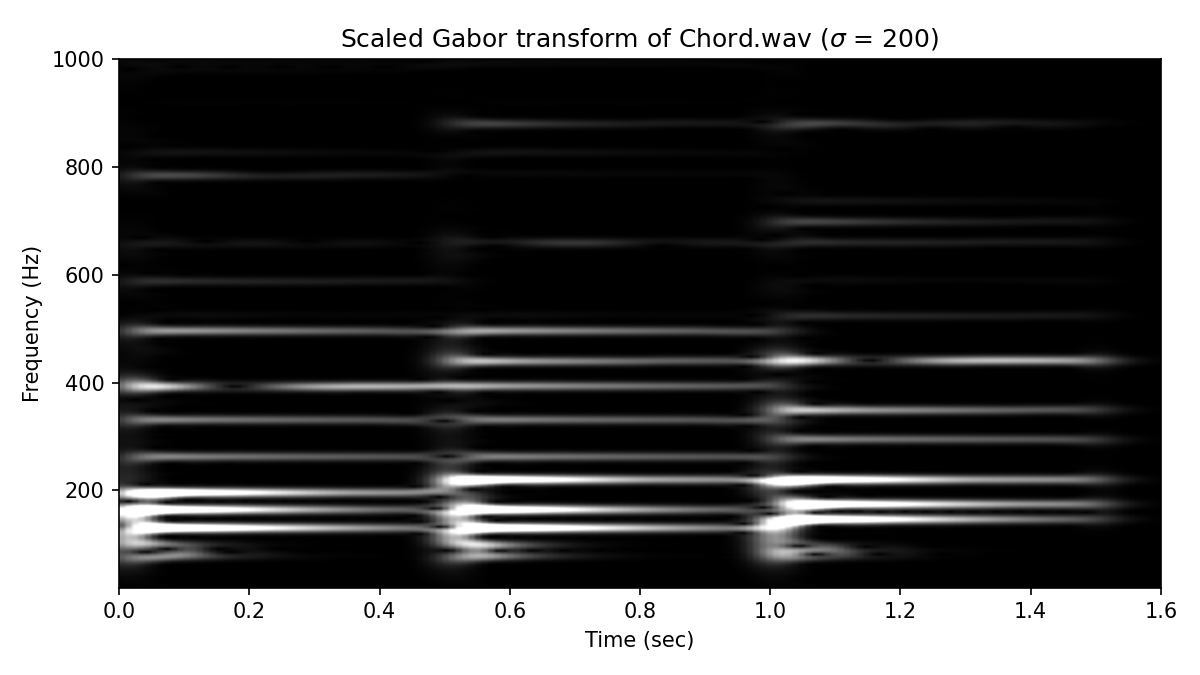
\includegraphics[width=0.9\textwidth]{Gabor_result.png}
\caption{Scaled Gabor transform of \texttt{Chord.wav} with $\sigma=200$.}
\end{figure}

The running time is $0.0417$ s.

%=====================================================================
\item (extra)
\begin{figure}[H]
\centering
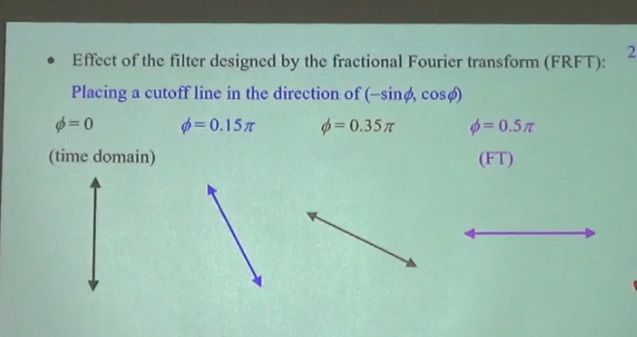
\includegraphics[width=0.9\textwidth]{extra.png}
\end{figure}

When $\phi=0.15\pi$, it is equivalent to performing the Fourier transform \textbf{0.3 times}.

The FRFT with angle $\phi$ is the LCT with $\begin{bmatrix}a&b\\c&d\end{bmatrix}=\begin{bmatrix}\cos\phi&\sin\phi\\-\sin\phi&\cos\phi\end{bmatrix}$, which rotates the WDF by $\phi$. The original FT corresponds to $\phi=\pi/2$, and the FRFT satisfies the additivity property
\[
O_F^{\phi_1}\big(O_F^{\phi_2}(x)\big)=O_F^{\phi_1+\phi_2}(x).
\]
Thus performing the FT $a$ times rotates the time-frequency plane by $a\cdot\frac\pi2$, i.e., the order of the FRFT is $a=\phi/(\pi/2)$. For $\phi=0.15\pi$,
\[
a=\frac{0.15\pi}{\pi/2}=0.3,
\]
so the FRFT with $\phi=0.15\pi$ is the 0.3-th order Fourier transform. Similarly, $\phi=0$ ($a=0$) is the time domain, $\phi=0.35\pi$ corresponds to $a=0.7$, and $\phi=0.5\pi$ ($a=1$) is the original FT.

\end{enumerate}

\end{document}